\documentclass[conference]{IEEEtran}
\IEEEoverridecommandlockouts

\usepackage{cite}
\usepackage{amsmath,amssymb,amsfonts}
\usepackage{algorithmic}
\usepackage{graphicx}
\usepackage{textcomp}
\usepackage{xcolor}
\usepackage{hyperref}
\def\BibTeX{{\rm B\kern-.05em{\sc i\kern-.025em b}\kern-.08em
    T\kern-.1667em\lower.7ex\hbox{E}\kern-.125emX}}







\pagestyle{plain}
\begin{document}
\title{
\makebox[0pt][l]{%
    \hspace*{-1.8cm}% décalage vers la gauche
    \raisebox{1.em}[0pt][0pt]{%
        
\includegraphics[width=0.20\textwidth]{logo_vnu.jpg}}%
}
\hspace{1.6cm}Self2Seg: Segmentation et D\'ebruitage Conjoints Auto-Supervis\'es d'une Seule Image\\
}

\author{\IEEEauthorblockN{Analysé par Ebwala Ebwalette Priscille}
\IEEEauthorblockA{\textit{\'Ecole Internationale, Institut Francophone International} \\
\textit{Universit\'e Nationale du Vietnam} \\
Bibiographie et Etude de Cas\\
Superviseur: \textbf{Dr. Ho Tuong Vinh}\\
Promotion: SIM P27\\
Sources : \href{https://fr.overleaf.com/read/pnghmnytwfvn#447962}{Lien vers le document partagé sur Overleaf}\\
version francais : articleFrancais.tex.
\\
version anglais : articleAnglais.tex.
}
}

\begin{document}

\maketitle

\begin{abstract}

Ce rapport est réalisé dans le cadre de l’unité d’enseignement intitulée \og Bibliographie et Étude des cas \fg{}. L’objectif est de permettre à l’étudiant de mener une étude approfondie d’un article scientifique. L’article analysé, intitulé \textit{Self2Seg : Segmentation et débruitage conjoints auto-supervisés d’une seule image}, propose une méthode novatrice permettant de segmenter et de débruiter une image simultanément, sans nécessiter de données annotées. Les auteurs soulignent dans un premier temps les limites des approches traditionnelles, qui traitent ces deux tâches séparément et dépendent fortement de jeux de données étiquetés. Pour surmonter ces limites, l’article présente une approche conjointe, basée sur des réseaux neuronaux auto-supervisés et une fonction énergétique partagée entre les deux tâches. Cette solution repose sur l’utilisation d’experts de débruitage spécifiques aux régions de l’image, permettant une interaction dynamique entre les étapes de segmentation et de débruitage. Les auteurs détaillent ensuite l’architecture de leur modèle, sa mise en œuvre, ainsi que les résultats expérimentaux obtenus sur des images biomédicales bruitées. L’article se termine par des perspectives d’amélioration de la méthode et d’extension à d’autres domaines d’application.
\end{abstract}

\end{abstract}

\begin{IEEEkeywords}
Segmentation, d\'ebruitage, auto-supervision, images biom\'edicales, apprentissage profond, Self2Seg
\end{IEEEkeywords}

\section{Introduction}
La segmentation et le débruitage d’images sont deux étapes fondamentales en vision par ordinateur, notamment dans le domaine biomédical où l’analyse précise des structures est cruciale. Traditionnellement, ces deux tâches sont traitées séparément à l’aide de modèles supervisés qui exigent un grand volume de données annotées. Cette dépendance aux annotations représente un obstacle important, notamment dans des contextes où les données labellisées sont rares ou coûteuses à obtenir.
Dans l’objectif de surmonter ces limitations, des approches auto-supervisées ont récemment émergé, permettant de s’affranchir partiellement ou totalement de l’usage de vérités terrain. Parmi elles, certaines intègrent des techniques de débruitage auto-supervisé telles que \textit{Noise2Self}, tandis que d’autres s’attaquent à la segmentation par des modèles non supervisés.
L’article étudié dans le cadre de ce module d'enseignement \fg{} présente une solution novatrice nommée \textit{Self2Seg}, qui combine de manière conjointe et auto-supervisée la segmentation et le débruitage d’une image. Les auteurs proposent un modèle basé sur une fonction énergétique commune et sur des réseaux neuronaux spécialisés pour chaque région de l’image (avant-plan et arrière-plan). Ce protocole permet non seulement d’améliorer la qualité des images traitées mais aussi la précision des segmentations obtenues, sans recours à des annotations manuelles.
Ce rapport vise à résumer de manière structurée l’approche proposée, à en analyser la mise en œuvre, à discuter les résultats expérimentaux, et à mettre en perspective cette solution au regard des travaux connexes dans le domaine.

\section{CONTEXTE, PROBLÉMATIQUE ET OBJECTIFS DE L'ARTICLE}

Ce travail s’inscrit à la croisée du traitement d’image, de l’apprentissage profond et de l’optimisation sans supervision. Les auteurs y explorent la segmentation et le débruitage d’images dans un cadre auto-supervisé, à travers la méthode \textit{Self2Seg}. La segmentation vise à identifier les régions pertinentes d’une image, tandis que le débruitage réduit les perturbations visuelles, telles que le bruit gaussien. Ces deux tâches sont particulièrement cruciales en imagerie biomédicale, où la qualité des données conditionne la fiabilité des analyses. Cependant, leur efficacité repose souvent sur des annotations manuelles, coûteuses et parfois indisponibles. De plus, les méthodes classiques les traitent séparément, empêchant une exploitation mutuelle de leurs bénéfices.

Face à cette problématique, les auteurs posent une question centrale : \textit{comment segmenter et débruiter efficacement une image à partir d’un seul échantillon non annoté ?} Pour y répondre, ils proposent une approche conjointe auto-supervisée, basée sur une optimisation croisée entre les deux processus.

L’objectif principal de l’article est donc de concevoir une méthode robuste et synergique, capable de réduire la dépendance aux vérités terrain. Les résultats montrent que cette approche améliore à la fois la qualité des images restaurées et la précision des segmentations, en particulier dans des contextes fortement bruités et sans annotations disponibles.

\section{\'Etat de l’Art}

Les auteurs de l’article ont mené un état de l’art approfondi afin d’identifier les approches existantes traitant de la segmentation et du débruitage d’images, en particulier dans un cadre auto-supervisé. Trois axes de recherche principaux ont été explorés : \textbf{les méthodes variationnelles, le débruitage par apprentissage profond, et les approches combinées.}Premièrement, les méthodes variationnelles, comme l’approche de Chan-Vese et ses variantes, ont été utilisées pour segmenter des images tout en atténuant le bruit. Bien qu’efficaces, elles nécessitent souvent un prétraitement et ne s’adaptent pas bien aux images fortement bruitées ou non annotées. Deuxièmement, des techniques comme \textit{Noise2Self}, \textit{Noise2Void} et \textit{Noise2Fast} permettent un débruitage auto-supervisé sans avoir besoin de données annotées. Toutefois, elles se concentrent sur la qualité visuelle sans intégrer de composantes de segmentation. Troisièmement, certaines recherches ont tenté de combiner les deux tâches. Par exemple, \textit{DenoiSeg} utilise un réseau U-Net pour segmenter et débruiter en parallèle, mais dépend toujours de masques partiels.

Face à ces constats, les auteurs de \textit{Self2Seg} soulignent les limites des travaux existants, notamment l’absence d’un cadre unifié et auto-supervisé capable de combiner efficacement les deux tâches sans annotations. Leur méthode vise à surmonter ces lacunes en exploitant l’interaction mutuelle entre segmentation et débruitage dans un processus d’optimisation conjointe.


\section{ SOLUTION PROPOSÉE }

Dans leur article, les auteurs proposent, avec \textit{Self2Seg}, un modèle dans lequel le débruitage et la segmentation sont étroitement liés. L'idée centrale repose sur l’optimisation conjointe d’une fonction énergétique, où chaque tâche influence et renforce l’autre.

\subsection{\textbf{ Débruitage spécifique à une région }}

 Deux réseaux neuronaux indépendants sont entraînés pour traiter respectivement les régions de l’avant-plan (DF) et de l’arrière-plan (DB). Ces réseaux, appelés \og experts \fg{}, possèdent leurs propres paramètres (notés F et B) et sont entraînés selon une stratégie de débruitage adaptée à chaque type de région. Bien que le modèle soit initialement présenté pour deux régions, son extension à plusieurs classes reste simple et s’appuie sur des travaux antérieurs.
    \begin{figure}[htbp]
        \centering
        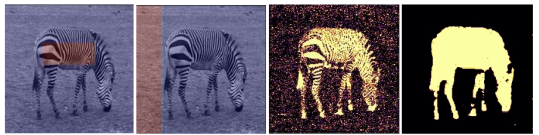
\includegraphics[width=0.4\textwidth]{debruit_region.png}
        \caption{Illustration du processus : image d’entrée, détection des régions par les débruiteurs, puis masque de segmentation obtenu après optimisation.}

        \label{fig:debruitage_regions}
    \end{figure}
    
\subsection{\textbf{Couplage des deux tâches}}
La segmentation et le débruitage sont considérées comme interdépendantes. Leur traitement simultané au sein d’un même cadre d’optimisation permet d’améliorer significativement la qualité des résultats. Les auteurs identifient trois aspects fondamentaux de cette interaction :

\begin{itemize}
    \item Influence de la segmentation sur le débruitage : En s'appuyant sur les cartes de segmentation, le modèle cible plus efficacement les zones d’intérêt, ce qui permet un débruitage plus précis sans altérer les détails importants.
    
    \item Influence du débruitage sur la segmentation : En améliorant la qualité visuelle des images, le débruitage facilite la détection des objets et des contours, rendant les segmentations plus nettes et plus robustes aux variations de bruit.

    \item Optimisation conjointe : Contrairement aux méthodes séquentie{-}lles, Self2Seg repose sur une fonction énergétique partagée qui pilote simultanément les deux processus. Ce couplage favorise un apprentissage plus cohérent et un échange d’informations continu entre les deux modules.
\end{itemize}


\begin{figure}[htbp]
    \centering
    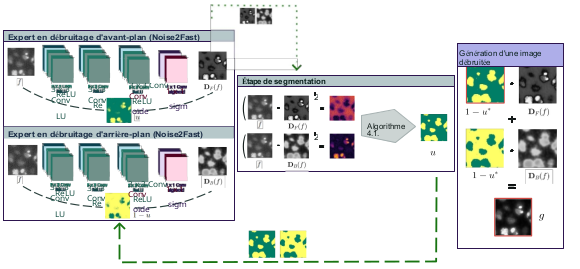
\includegraphics[width=0.4\textwidth]{couplage_deux_taches.png}
    \caption{Schéma illustrant l’interaction entre les experts en débruitage pour les différentes régions de l’image et le processus de segmentation, dans le cadre du modèle Self2Seg.}
    \label{fig:couplage_self2seg}
\end{figure}
Grâce à cette synergie, \textit{Self2Seg} surpasse les approches traditionnelles en exploitant pleinement l'interaction entre les deux tâches. Cette stratégie rend le modèle plus robuste, plus général, et mieux adapté aux situations où les annotations sont absentes.

\section{MISE EN ŒUVRE ET EXPERIMENTATION DE L'ARTICLE}

\subsection{\textbf{ Mise en œuvre}}

La mise en œuvre de la méthode \textit{Self2Seg} repose sur un processus structuré en plusieurs étapes clés :

\subsubsection{\textbf{Discrétisation et initialisation }}\\

La procédure débute par la discrétisation de l’image et la définition de masques de segmentation initiaux. Ces masques peuvent être obtenus soit par seuillage automatique des intensités, soit par la sélection manuelle de boîtes délimitant les régions représentatives de l’avant-plan et de l’arrière-plan. Les experts en débruitage, notés $D_F$ (pour l’avant-plan) et $D_B$ (pour l’arrière-plan), sont ensuite entraînés à partir de ces masques initiaux afin d’apprendre des caractéristiques spécifiques à chaque type de région.

\subsubsection{\textbf{Optimisation alternée }}\\

 Le processus d’optimisation s’effectue de manière itérative, en alternant entre la mise à jour des experts en débruitage et celle du masque de segmentation. L’optimiseur ADAM est utilisé pour entraîner les réseaux de débruitage jusqu’à convergence. Lorsque les paramètres des réseaux sont figés, la fonction énergétique est minimisée afin d’ajuster le masque de segmentation. Cette étape d’optimisation est réalisée à l’aide de l’algorithme primal-dual de Chambolle-Pock.

\subsubsection{\textbf{Critère de convergence }}\\

  Les itérations se poursuivent jusqu’à ce que la diminution relative de l’énergie tombe en dessous de 15~\% par rapport à l’itération précédente, garantissant ainsi un compromis satisfaisant entre efficacité computationnelle et qualité du résultat final.
    


\subsection{\textbf{ Expérimentation}}

\subsubsection{\textbf{Données et métriques}}\\
 Les expériences sont menées sur le jeu de données de noyaux cellulaires issu du défi \textit{Kaggle 2018 Data Science Bowl (DSB2018)}.Les images sont volontairement dégradées par un bruit gaussien avec des niveaux de variance croissants : 10, 30 et 50. Ainsi Les performances sont évaluées selon trois indicateurs : l’indice de Dice pour la segmentation, la similarité structurelle (SSIM) et le rapport signal-bruit maximal (PSNR) pour le débruitage.
   
\subsubsection{\textbf{Comparaison des méthodes}}\\
    La méthode \textit{Self2Seg} est comparée à plusieurs approches de référence, dont le modèle convexe de Chan-Vese, une méthode séquentielle basée sur \textit{Noise2Fast}, ainsi qu’un modèle à apprentissage profond nommé \textit{DenoiSeg}. Les auteurs, en comparant cette methode avec les differents approches,Les résultats expérimentaux montrent que \textit{Self2Seg} surpasse ces approches concurrentes, notamment dans les conditions les plus bruitées, avec des performances mesurées par les métriques suivantes :
        \begin{itemize}
            \item \hspace{0.5em}\textbf{PSNR} (Peak Signal-to-Noise Ratio) : mesure de la qualité du débruitage ;
            \item \hspace{0.5em}\textbf{SSIM} (Structural Similarity Index) : évalue la fidélité visuelle de l’image restaurée ;
            \item \hspace{0.5em}\textbf{Indice de Dice} : évalue la précision de la segmentation.
        \end{itemize}
    
\subsubsection{\textbf{Résultats expérimentaux }}\\

Les auteurs ont évalué les performances de leur méthode \textit{Self2Seg} dans différents scénarios de bruit afin de mesurer sa robustesse et sa capacité d’adaptation. Les résultats obtenus mettent en évidence la pertinence de l’approche, aussi bien sur des images faiblement bruitées que dans des contextes plus dégradés. Plusieurs observations clés ressortent des expérimentations :
\begin{itemize}
    \item Pour un niveau de bruit faible (variance = 10), un seul expert en débruitage est utilisé, en partant de l’hypothèse d’un arrière-plan homogène. Dans ce cas, la méthode permet déjà d’obtenir des segmentations nettes et précises.
    
    \item Pour des niveaux de bruit plus élevés (variance = 30 et 50), les auteurs mobilisent deux experts en débruitage, associés à un filtrage spécifique du terme de fidélité pour l’arrière-plan. Cette stratégie permet d’éviter la sur-segmentation et de stabiliser le masque produit.

    \item De manière générale, les résultats montrent que \textit{Self2Seg} surpasse les méthodes de référence, aussi bien en termes de qualité visuelle qu’en performance quantitative. L’approche se distingue notamment dans les régions complexes des images bruitées, en produisant des segmentations plus précises et des reconstructions d’images plus fidèles.
\end{itemize}

\subsubsection{\textbf{Extensions et limitations }}\\
    
       Le modèle peut être généralisé à des tâches de segmentation multiclasse en intégrant plusieurs experts spécialisés. Une limitation est observée lorsque l’un des débruiteurs couvre partiellement les deux régions cibles, ce qui peut entraîner une mauvaise convergence des masques. Une stratégie de contrainte est proposée pour atténuer ce phénomène. L’intégration de variantes comme le \textit{deep image prior} est également suggérée afin de renforcer la robustesse dans certains cas spécifiques.
    


Ainsi, les auteurs proposent avec \textit{Self2Seg} une approche robuste alliant modèles variationnels et apprentissage profond auto-supervisé, offrant des résultats efficaces en segmentation et débruitage, même dans des conditions de bruit élevé.

\section{ ARTICLES CONNEXES}

Dans le domaine de l’auto-supervision appliquée à la segmentation et au débruitage, plusieurs travaux connexes proposent des approches complémentaires à \textit{Self2Seg}. Ces études partagent le même objectif : réduire la dépendance aux annotations manuelles tout en améliorant la performance des modèles en vision par ordinateur.

\subsubsection{\textbf{BEVContrast: Self-Supervision in BEV Space for Automotive Lidar Point Clouds [2] }}\\ 
    Les auteurs présentent une méthode basée sur l’apprentissage contrastif appliqué aux nuages de points LiDAR, dans une vue en \textit{Bird’s Eye View} (BEV). Cette approche permet une segmentation améliorée tout en limitant les besoins en annotations. Toutefois, elle reste spécifiquement conçue pour la perception autonome et n’est pas directement applicable aux images microscopiques, comme celles ciblées par \textit{Self2Seg}.
     \begin{figure}[htbp]
    \centering
    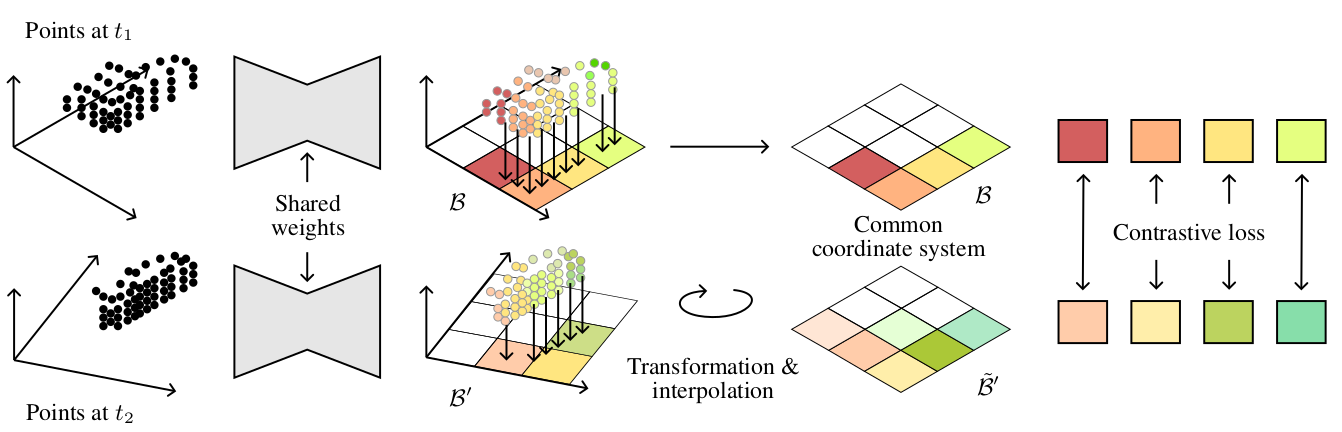
\includegraphics[width=0.4\textwidth]{article_1.png}  % Remplace par le nom de ton image
    \caption{Architecture du système }
    \label{fig:monimage}
\end{figure}

\subsubsection{\textbf{Multi-Task Self-Supervised Learning for Image Segmentation Task [3] }}\\

    Cette méthode propose un apprentissage auto-supervisé multitâche intégrant la segmentation sémantique, la prédiction de profondeur et la normalisation de surface. Elle améliore la robustesse globale du modèle. Cependant, le compromis entre les différentes tâches peut nuire à la précision de la segmentation, surtout lorsque les objectifs sont fortement interdépendants.
%       \begin{figure}[htbp]
%     \centering
%     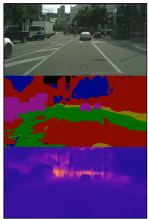
\includegraphics[width=0.1\textwidth]{article2.png}  % Remplace par le nom de ton image
%     \caption{Visualisation de résultat}
%     \label{fig:monimage}
% \end{figure}

\subsubsection{\textbf{Source Identification: A Self-Supervision Task for Dense Prédiction [4]  }}\\
    
    Inspirée des techniques de séparation aveugle des sources, cette approche vise à reconstruire des images originales à partir de compositions synthétiques. Elle s’est révélée efficace dans le contexte de l’imagerie médicale, mais son application reste encore limitée à d’autres domaines.
      \begin{figure}[htbp]
    \centering
    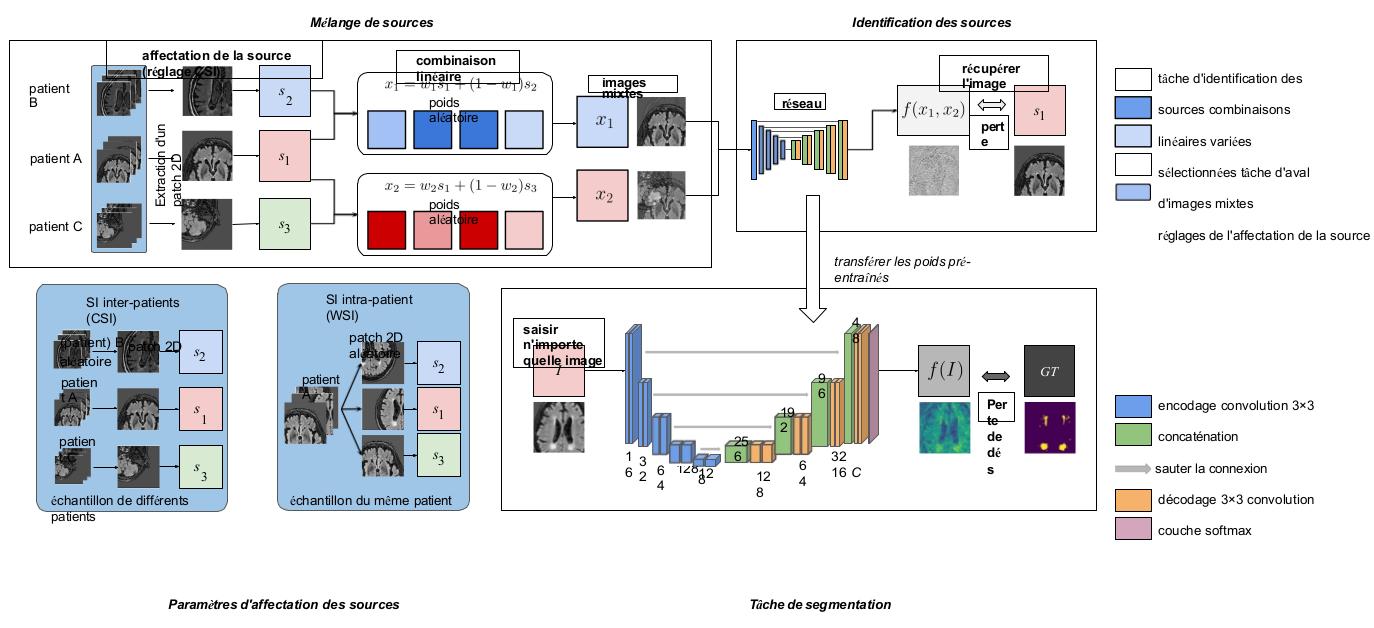
\includegraphics[width=0.4\textwidth]{article_3.png}  % Remplace par le nom de ton image
    \caption{Illustration de la tâche d’identification de source à partir de trois images, utilisant des stratégies inter- et intra-patients (CSI et WSI), avec des opérations de sous- et suréchantillonnage appliquées dans l’architecture UNet.}

    \label{fig:monimage}
\end{figure}

Ces travaux montrent que l’apprentissage auto-supervisé peut s’adapter à divers contextes et tâches en vision par ordinateur. Toutefois, \textit{Self2Seg} se distingue par son couplage explicite entre la segmentation et le débruitage dans un cadre entièrement auto-supervisé, ce qui constitue un avantage notable pour les applications exigeant des segmentations précises sans annotations manuelles.

\section{7. CRITIQUE PERSONNELLE DE L'ARTICLE}

L’article \textit{Self2Seg} présente une contribution intéressante dans le domaine de la vision par ordinateur. Après une analyse approfondie, plusieurs éléments ressortent, tant du point de vue des forces que des limites et des perspectives d’amélioration.

\subsection{\textbf{ Points forts}}
\begin{itemize}
    \item \hspace{0.5em}\textbf{Approche innovante :} L’intégration conjointe du débruitage et de la segmentation dans un cadre entièrement auto-supervisé constitue une avancée notable par rapport aux méthodes classiques, souvent séquentielles et fortement dépendantes d’annotations.

    \item \hspace{0.5em}\textbf{Indépendance aux données annotées :} Le modèle peut être entraîné sans vérités terrain, ce qui le rend particulièrement adapté aux domaines comme l’imagerie biomédicale, où les annotations sont rares, coûteuses ou difficiles à obtenir.

    \item \hspace{0.5em}\textbf{Robustesse face au bruit :} Les expérimentations ont démontré l’efficacité de \textit{Self2Seg} dans des conditions de bruit élevé, surpassant plusieurs méthodes de référence sur des images fortement dégradées.
\end{itemize}

\subsection{\textbf{Limites}}
\begin{itemize}
    \item \hspace{0.5em}\textbf{Sensibilité aux hyperparamètres :} La performance du modèle dépend fortement du choix des hyperparamètres, ce qui peut rendre sa mise en œuvre complexe sans un réglage adapté ou automatisé.

    \item \hspace{0.5em}\textbf{Portabilité limitée :} Bien que performante sur des images microscopiques, la méthode pourrait nécessiter des ajustements pour être généralisée à d'autres types d’images, notamment dans des contextes industriels ou naturels.

    \item \hspace{0.5em}\textbf{Comparaison incomplète :} L’évaluation aurait gagné en pertinence si les auteurs avaient confronté leur modèle à des architectures de segmentation plus récentes et performantes, comme les modèles à base de Transformers ou d’autoencodeurs avancés.
\end{itemize}

\subsection{\textbf{ Perspectives d’amélioration}}
\begin{itemize}
    \item \hspace{0.5em}\textbf{Généralisation à d’autres domaines :} Tester le modèle sur des jeux de données issus de la vision industrielle, de l’imagerie satellitaire ou de la photographie naturelle permettrait de valider sa robustesse hors du domaine biomédical.

    \item \hspace{0.5em}\textbf{Optimisation automatisée :} L’intégration de techniques comme l’AutoML ou la recherche bayésienne d’hyperparamètres pourrait faciliter le déploiement du modèle en réduisant la phase de calibration manuelle.

    \item \hspace{0.5em}\textbf{Hybridation avec d’autres approches :} Fusionner \textit{Self2Seg} avec des stratégies complémentaires, telles que l’apprentissage contrastif ou le multitâche, pourrait renforcer la qualité des représentations apprises et améliorer la performance globale.
\end{itemize}

\section{Conclusion}

L’article \textit{Self2Seg} apporte une contribution notable au domaine du traitement d’image en proposant une méthode auto-supervisée intégrant simultanément le débruitage et la segmentation. En éliminant le besoin en annotations manuelles, cette approche constitue une avancée pertinente, en particulier pour les applications en imagerie biomédicale où les données étiquetées sont souvent limitées. Le modèle se distingue par sa robustesse face au bruit, sa flexibilité d’adaptation, et son efficacité démontrée à travers plusieurs scénarios expérimentaux. L’analyse de cet article a permis de développer des compétences en lecture critique, en synthèse d’approches scientifiques et en évaluation comparative de méthodes. Elle a également favorisé une meilleure compréhension des enjeux actuels liés à l’apprentissage auto-supervisé, notamment dans le contexte de la segmentation d’images bruitées. Ce travail s’inscrit ainsi dans une démarche de réflexion approfondie sur les solutions innovantes en vision par ordinateur.


\begin{thebibliography}{00}
\bibitem{b1} N. Gruber, J. Schwab, N. Debroux, N. Papadakis, and M. Haltmeier, 
“Self2Seg: Single-Image Self-Supervised Joint Segmentation and Denoising,” 
\textit{arXiv preprint arXiv:2309.10511}, 2024.

\bibitem{b2} C. Sautier, G. Puy, A. Boulch, R. Marlet, and V. Lepetit, 
“BEVContrast: Self-Supervision in BEV Space for Automotive Lidar Point Clouds,” 
in \textit{arXiv:2310.17281v1 [cs.CV]}, 2023.

\bibitem{b3} L. Gao, C. Khamesra, U. Kumbhar, and A. Aglawe, 
“Multi-Task Self-Supervised Learning for Image Segmentation Task,” 
in \textit{arXiv:2302.02483v1 [cs.LG]}, 2023.

\bibitem{b4} S. Chen, S. Kayal, and M. de Bruijne, 
“Source Identification: A Self-Supervision Task for Dense Prediction,” 
\textit{arXiv:2307.02238v1 [cs.CV]}, 2023.

\end{thebibliography}

\end{document}
